
\documentclass[border=5pt]{standalone}
\usepackage[utf8]{inputenc}
\usepackage[T1]{fontenc}
\usepackage{amsmath,amssymb}
\usepackage{tikz}
\usetikzlibrary{arrows.meta,shapes.misc,calc}
\renewcommand{\familydefault}{\sfdefault}
\tikzset{
  ptcross/.style={cross out,draw,thick,minimum size=1.6mm,inner sep=0pt},
  vec/.style={->,thick,>={Stealth[length=2.6mm]}},
  vecu/.style={vec,color=blue!70!black},
  vecv/.style={vec,color=red!75!black},
  vecw/.style={vec,color=green!45!black},
  grid/.style={gray!35,thin},
}
\newcommand{\Vj}[1]{\overrightarrow{\text{#1}}}
\newcommand{\pt}[4]{\node[ptcross] at (#1,#2) {}; \node[anchor=#4,inner sep=2pt] at (#1,#2) {$#3$};}
\begin{document}
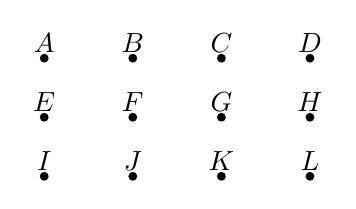
\begin{tikzpicture}[x=0.75cm,y=0.75cm]
\fill (0.0,2) circle (1.6pt); \node[anchor=south,inner sep=2pt] at (0.0,2) {$A$};
\fill (1.5,2) circle (1.6pt); \node[anchor=south,inner sep=2pt] at (1.5,2) {$B$};
\fill (3.0,2) circle (1.6pt); \node[anchor=south,inner sep=2pt] at (3.0,2) {$C$};
\fill (4.5,2) circle (1.6pt); \node[anchor=south,inner sep=2pt] at (4.5,2) {$D$};
\fill (0.0,1) circle (1.6pt); \node[anchor=south,inner sep=2pt] at (0.0,1) {$E$};
\fill (1.5,1) circle (1.6pt); \node[anchor=south,inner sep=2pt] at (1.5,1) {$F$};
\fill (3.0,1) circle (1.6pt); \node[anchor=south,inner sep=2pt] at (3.0,1) {$G$};
\fill (4.5,1) circle (1.6pt); \node[anchor=south,inner sep=2pt] at (4.5,1) {$H$};
\fill (0.0,0) circle (1.6pt); \node[anchor=south,inner sep=2pt] at (0.0,0) {$I$};
\fill (1.5,0) circle (1.6pt); \node[anchor=south,inner sep=2pt] at (1.5,0) {$J$};
\fill (3.0,0) circle (1.6pt); \node[anchor=south,inner sep=2pt] at (3.0,0) {$K$};
\fill (4.5,0) circle (1.6pt); \node[anchor=south,inner sep=2pt] at (4.5,0) {$L$};

\end{tikzpicture}
\end{document}
